\chapter{\label{chap:ai}Algoritmos de Inteligência Artificial para Elevadores}

Neste capítulo vamos apresentar:

\begin{itemize}
\item Os detalhes dos algoritmos selecionados e justificar a suas escolhas perante o problema;
\item Introduzir o modelo de simulação do sistema~-~ou seja, a modelagem
prédio/andares/elevadores (e não a modelagem do simulador propriamente dito);
\item Detalhes de cada algoritmo e descrever como esperamos que seja o resultado de seu uso junto ao sistema.
\end{itemize}

% TODO: Mais introdução
A literatura fala em alguns algoritmos utilizados para a escolha de qual
elevador atenderá um pedido. Alguns deles são triviais e não devem ser
enquadrados no termo Inteligência Artificial, no entanto, sua implementação é
interessante, no mínimo para fins de comparação com os demais algoritmos.
% TODO: Referências

Conforme os algoritmos vão ficando mais complexos, mais dados são necessários.
Em um mundo perfeito, ter-se-ia todos os dados de cada passageiro~-~\textit{i.e.} cada
pessoa que chegasse ao elevador informaria de antemão para qual andar deseja ir.
No entanto, isto não é realista nos sistemas atuais. Portanto, os algoritmos
aqui descritos tentam fazer inferências a respeito de dados que não possuem,
quando relevante\footnote{\textit{e.g.} Podemos estimar a lotação do elevador
  com base no peso reportado pela balança interna do elevador, que já se
  encontra nele por motivos de segurança.}, ou tentar tomar decisões ignorando
os dados que não estão disponíveis.

\section{\label{sec:ai:nn}Nearest Neighbour}

O algoritmo de \textit{Nearest Neighbour} é o mais ingênuo de todos, e servirá
de base para a avaliação dos demais algoritmos.

Seu funcionamento é trivial: o elevador mais próximo do chamado sempre
atenderá este chamado.

Um dos muitos problemas deste algoritmo é que ele pode causar muitas mudanças de
direção de um elevador, o que acarreta num tempo de espera maior para os
passageiros dele.

O único propósito deste algoritmo é servir de base de comparação com outros
algoritmos propostos, de modo a validarmos o simulador. Espera-se que uma
melhora clara de desempenho seja notado ao comparar-se este com o próximo dos
mais triviais, o \textit{Nearest Neighbour Melhorado}.

% TODO: Quem fala nele?

\section{\label{sec:ai:nnm}Nearest Neighbour Melhorado}

Uma melhoria que pode ser feita ao algoritmo de \textit{Nearest Neighbour}
é considerar o sentido em que o elevador está indo para atender o chamado. Isto
implica em considerar-se agora a informação de sentido dos pedidos. É importante
notar que ainda não se considera quantas pessoas fizeram um pedido para qual
sentido~-~apenas sabe-se que há pedidos no andar, e como destinos tem-se ``para
cima'', ``para baixo'' ou ambos.

Este algoritmo resolve o problema de mudanças de direção que o algoritmo de
\textit{Nearest Neighbour} sofre.

No entanto, sua escolha para este trabalho também se dá para fim de comparação
com os outros e validação do simulador. Como seu comportamento é diferente do
caso mais trivial, mas ainda assim bastante simples, poderá ser visto com clareza
algum tipo de melhora no tempo de resposta do sistema simulado, bem como a validade do simulador.

\section{\label{sec:ai:minimize-cost-function}Minimização da Função de Custo}

O primeiro algoritmo de IA a ser testado é simples: define-se uma
função de custo, inerente a cada elevador, que descreve matematicamente quão
vantajoso é atender um pedido, comparado a não atendê-lo. A decisão de qual
elevador é escolhido para atender o pedido é feita com base única e
 exclusivamente em qual deles terá o menor valor da função de custo.

Um exemplo de função de custo é:

\[
  J(f) = \sum_{i=0}^{i=n} 2g_{i}f
\]

Onde $g_{i}$ é o tamanho do grupo dentro do elevador (que sabemos graça à
balança interna) e $f$ é a distância, em número de andares,
entre a posição atual do elevador e o pedido que se está avaliando. Note que,
caso haja uma mudança de direção, o valor de $f$ deve ser dobrado, pois o
elevador deverá ir até o novo pedido e então voltar para onde estava.

% TODO: Ilustração

Várias funções de custo podem ser experimentadas e comparadas.

Outras funções de custo levariam em consideração mudanças de direção de viagem
\footnote{\textit{e.g.}, pode ser vantajoso um elevador mudar de direção para atender um
pedido a um andar de distância, caso a alternativa seja fazer o pedido esperar
um deslocamendo de dezenas de andares de outro elevador.}, ou ainda tentar
manter todos os custos o mais baixo possível, ao mesmo tempo que sejam todos o
mais próximos uns dos outros.\footnote{É possível elevar cada termo do somatório ao
  quadrado para obter-se isto.}

% TODO: outros exemplos de função de custo?

\section{Planning}

% TODO: essa explicação pode melhorar ainda

A idéia do algoritmo de planning é estender o de função de custo, calculando a
mesma para vários passos no futuro~-~como em um jogo de xadrez.

O horizonte de cálculo deve ser selecionado, dado que é um fator limitante no
tamanho do cálculo do algoritmo.

Cada decisão diferente, para cada elevador, é um nodo novo na árvore. Ao
escolher-se uma das alternativas (\textit{i.e.} a que, ao final de $x$ eventos
no futuro tem o menor custo), avança-se um passo na simulação e executa-se o
algoritmo novamente.

Na Figura~\ref{fig:planning}, vemos um exemplo de planning sendo executado com
horizonte 3 e dois elevadores. Para cada passo do algoritmo, a decisão a ser
tomada é ``qual elevador deve atender o próximo pedido da fila?'', e, para isto,
calcula-se a função de custo. O resultado da função pode ser visto entre
parênteses em cada nodo da árvore da Figura~\ref{fig:planning}.

Ao encontrarmos o horizonte (no caso da Figura~\ref{fig:planning}, no nível 3 da
árvore), vemos quem tem o menor custo (neste caso, E2, filho de E2, filho de
E1). Toma-se então a decisão de descer um nível na árvore apenas, em direção ao
menor custo.

Veja que, ao fazer isto, poderá tomar-se uma decisão diferente do algoritmo que apenas
considera a função de custo. No caso da Figura~\ref{fig:planning}, o elevador E1
atenderá o próximo chamado, mesmo tendo um custo superior a E2.

\begin{figure}[htb!]
  \centering
  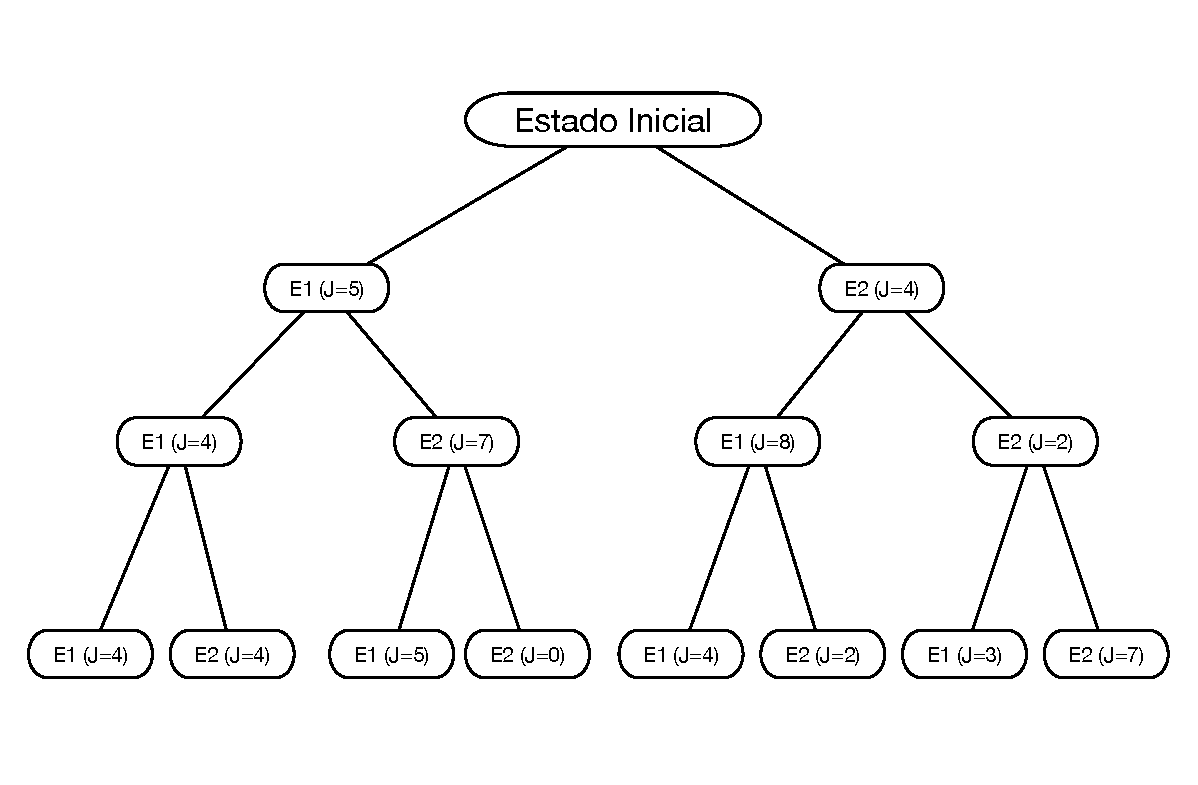
\includegraphics[scale=0.6]{img/planning.eps}
  \caption{Exemplo de planning com horizonte 3 e dois elevadores}
\label{fig:planning}
\end{figure}

\section{Planning Multi-Agente}

Este algoritmo é uma extensão do algoritmo de Planning, onde, em vez de termos
um processamento central que decide que um elevador deve atender o pedido, temos
todos os elevadores calculando por conta própria se vale a pena atender um
pedido ou não~-~sem conhecimento do estado dos demais.

A literatura neste tópico é bastante escassa ainda.